% remember to set these at the start of each chapter
\chapter{Background} 
\label{background} 

%%%%%%%%%%%%%%%%%%
Just for fun, you can see that acronyms are now redefined: \ac{est}.

\section{What About Figures}

Figures are dead easy to call. Just call them from within a Figure environment.

\begin{figure}[ht] % put figure roughly here, will float though
	\centering
	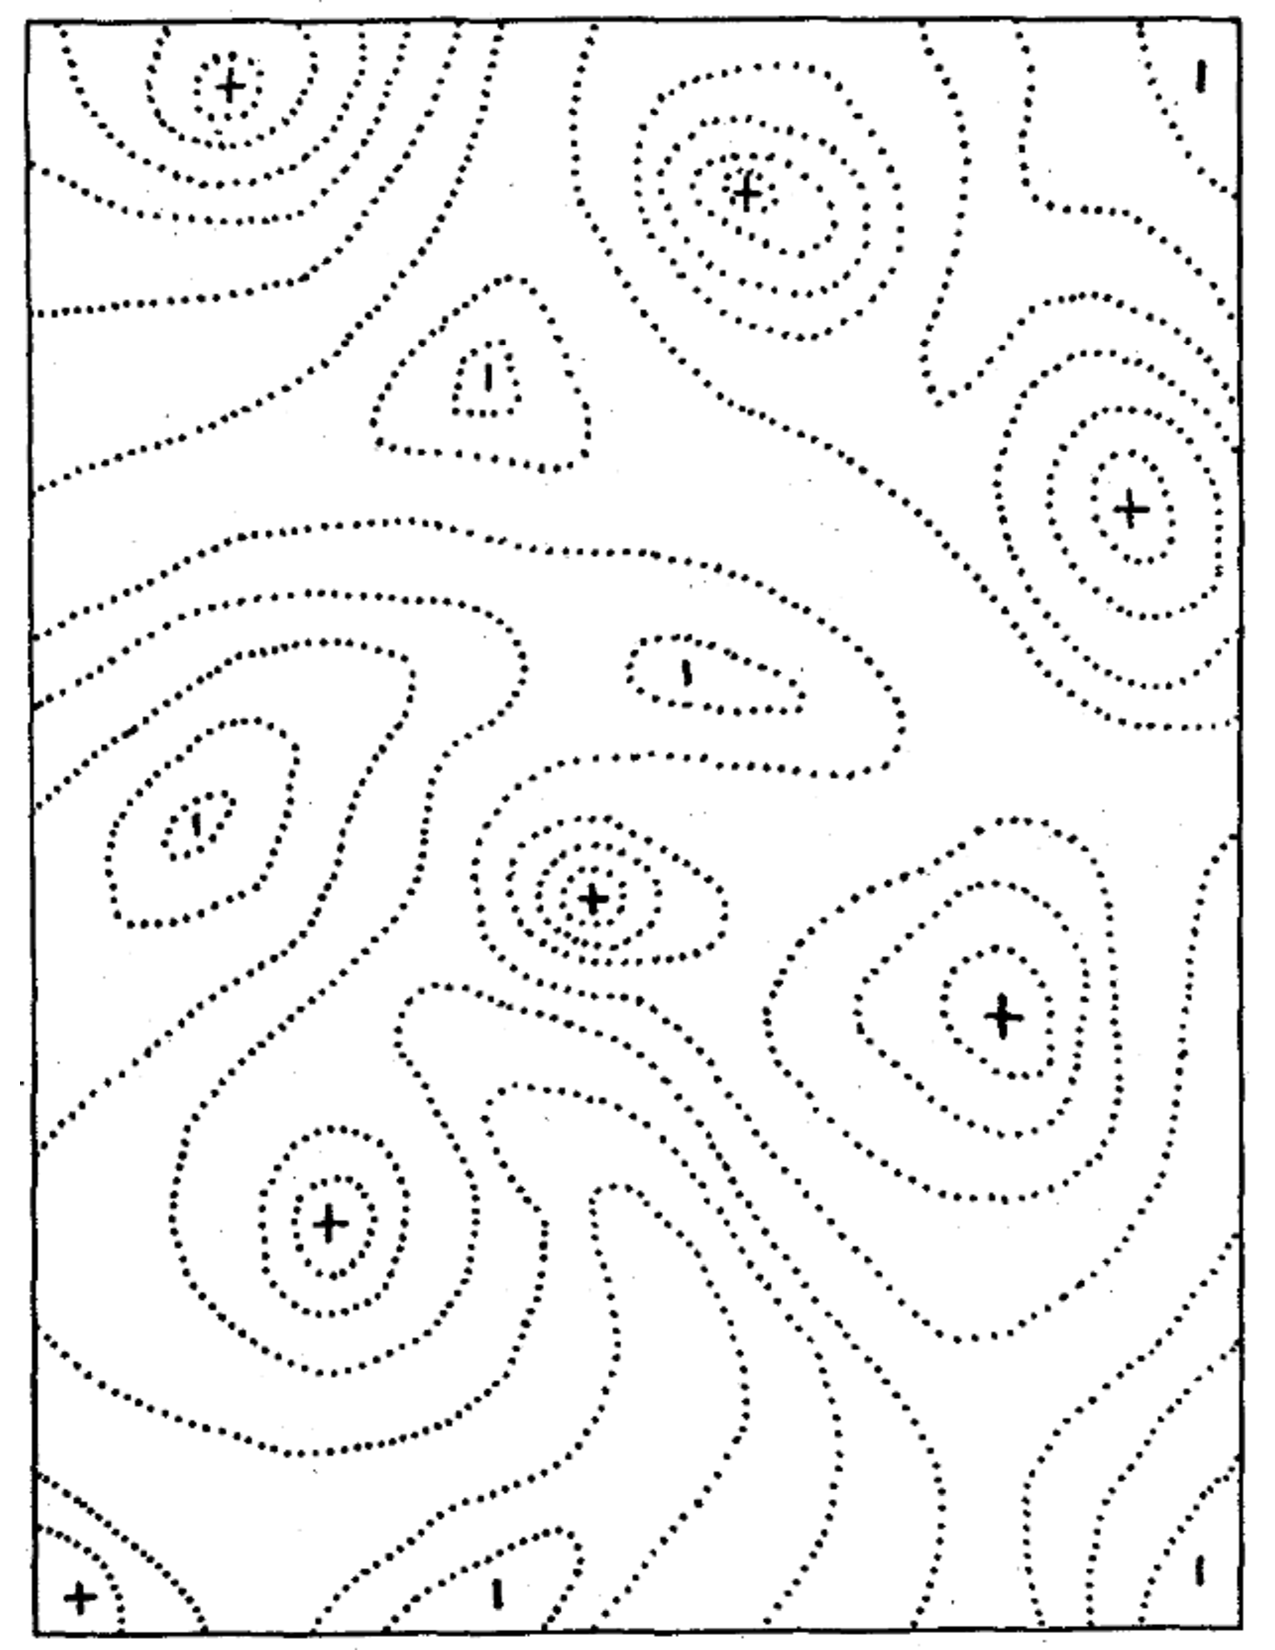
\includegraphics[width=0.5\textwidth]{Figs/Wright_1932_1.pdf}
    \caption[Adaptive landscape]{Early adaptive landscape sort of stuff}
    \label{landscape}
\end{figure}

And now, I do not need to remember the figure number. All I do is refer to the figure label that I gave it (Fig.\,\ref{landscape}). The size of figures can be controlled in the \verb+\includegraphics[]{}+ command. Above, I chose to make the figure 50\% of the width of the text on a page. I could alternatively put a specific dimension with \verb+width=85mm+ or even scale it to a some percentage of it's original size \verb+scale=0.5+ (in this case 50\% of its original size).  

As for my next figure, \LaTeX{} will automatically do the numbering. It will also attach the chapter number to the figure.



\begin{figure}[t] 
	\centering
	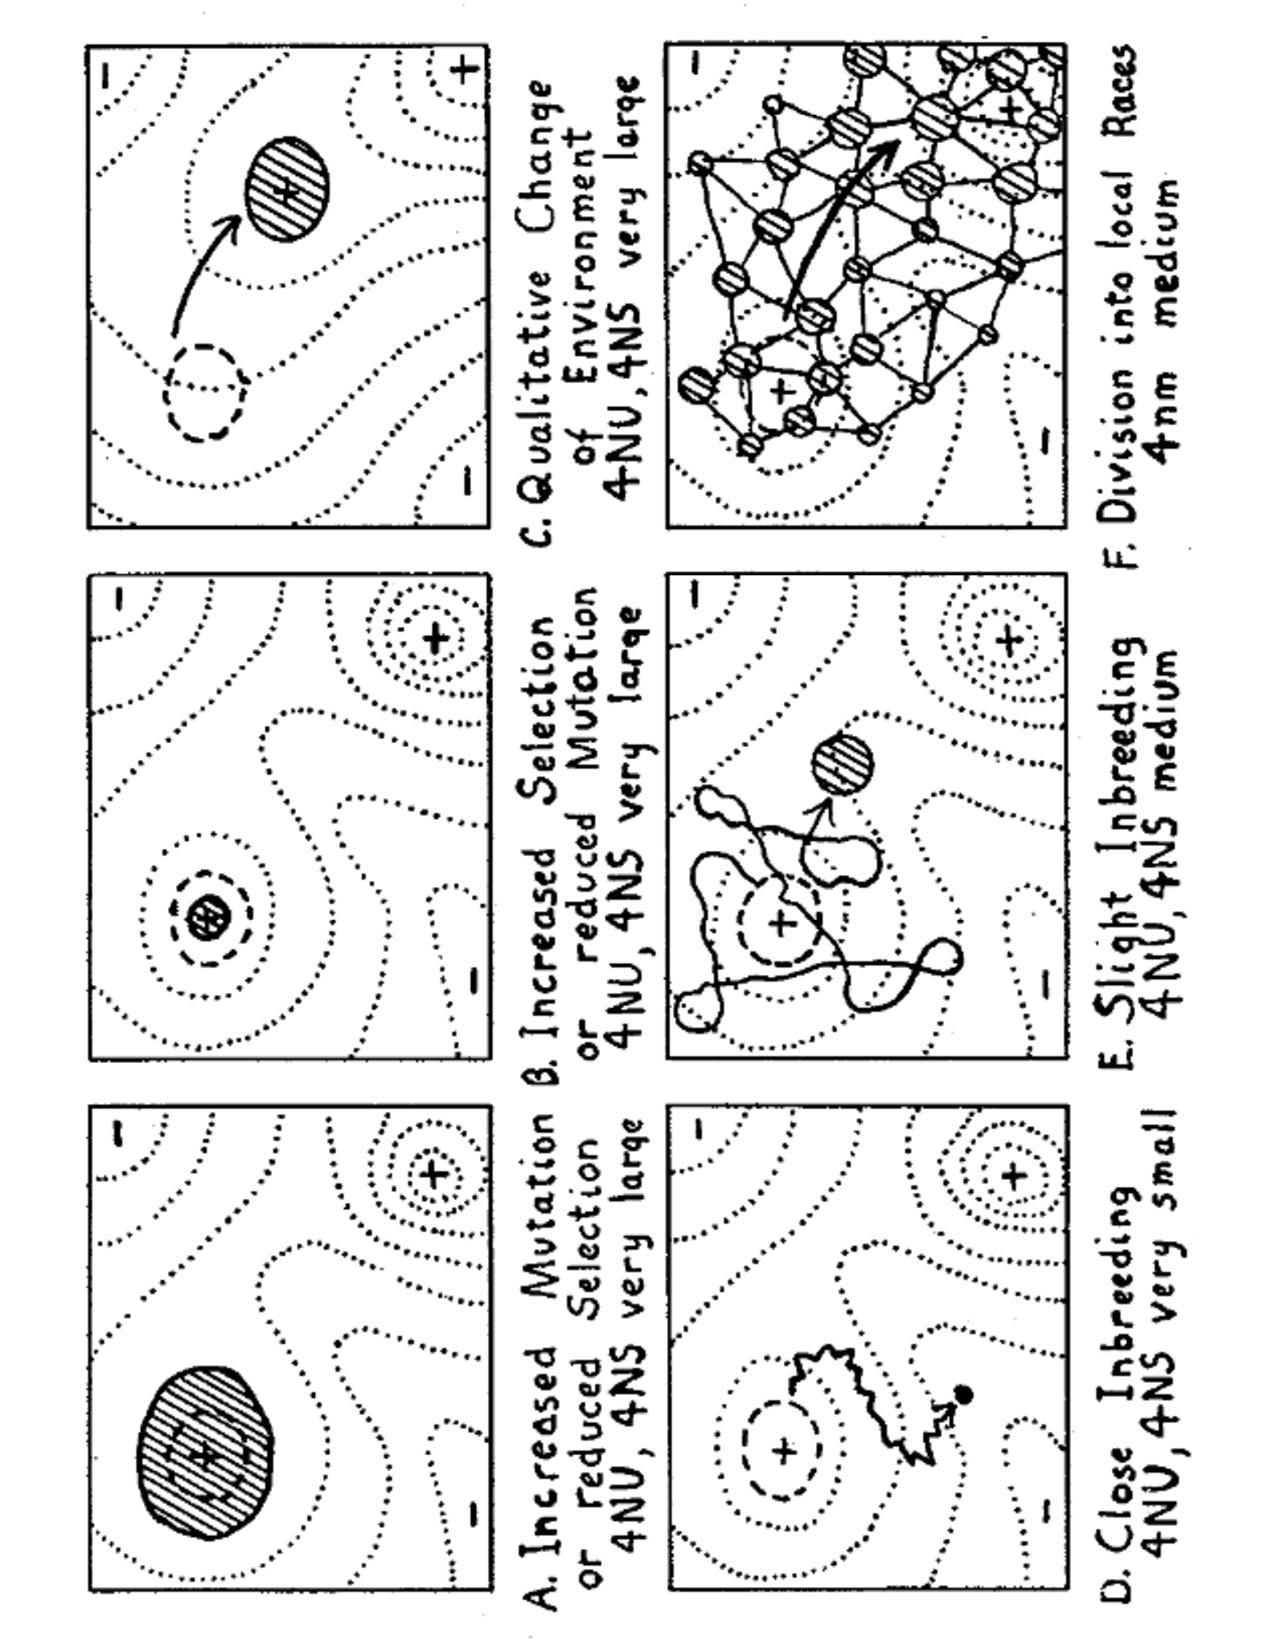
\includegraphics[scale=0.5, angle=-90]{Figs/Wright_1932_2.pdf}
    \caption[selection]{Wowza, glad I don't have to do figures by hand. Also, you may have noticed in the includegraphics command I rotated the image. If it was a multipage pdf you could also call specific pages}
    \label{bigFig}
\end{figure}

Then I will call it same as before (Fig.\,\ref{bigFig}). As you can see, it was placed on the next page, as \LaTeX{} thought that was best, given its size. Figures will float around, but you will never have to worry about numbering. One potential problem is that the figure placement may not end up the were want it to (not that you have to worry about getting the numbers wrong). You can suggest placement with the [h] after the \verb+\begin{figure}[h]+ and strongly suggest placement with [h!]. There are ways to force a figure placement, but do try and avoid forcing things (could end up looking weird). You can force positioning by putting \verb+\usepackage{float}+ in the preamble, then setting up the figure with a [H] like so: \verb+\begin{figure}[H]+. This stop the figure from floating.

You may notice the \verb+\,+ that just puts in a small space after the Fig ``period''. It's personal preference, and there are too many space options in \LaTeX{}. 


\section{Tables -- how to}

\subsection{Typing in Tables}
Small to medium tables I would suggest just typing it in to the \TeX{} file (see Table \ref{simpleTable} below). There are also packages to create \LaTeX{} tables (such as xtable in R) and packages to read in csv/tab files, like you read in figures. There are ways to make multi-column and multi-row values in tables; you will have to Google it (it is not hard to do). The \verb+\usepackage{multirow}+ will allow you to do multirow values. The command \verb+\multicolumn{}{}{}+ is already available. 

\begin{table}[h]
\centering
\caption[Simple table]{A simple typed in table. Note the special lines used in the table. Yes, typography rules call for different thickness of lines. The command \\hline will put in just a regular horizontal line}
\label{simpleTable}
\begin{tabular}{c|ccc} % a vertical bar here will put one in the table
\toprule
col1 & col2 & col3 & col4 \\
\midrule
1 & 2 & 3 & 4 \\
1 & 2 & \multicolumn{2}{c}{3} \\
\bottomrule
\end{tabular}
\end{table}



% reading in a csv file
\subsection{Reading in CSV table}

You can copy and paste the information into \LaTeX{} to keep things together, but it has to be dropped into the preamble in the main tex. Or you can call in the data file (Table \ref{csv_readin}).

Using \verb+\usepackage{pgfplotstable}+ is the package to use.

\begin{table}[h]
\centering
\caption[Normal size table]{Reading in a table}
\label{csv_readin}
\pgfplotstabletypesetfile[col sep=comma,every last row/.style={after row=\bottomrule},every head row/.style={before row={\toprule}, after row={\midrule}}]{Tables/Suppl_Table_1.csv}
\end{table}

If tables do not fit, you can shrink them by wrapping in a box or shrinking text (Table \ref{csv_readin_small}).

\begin{table}[h]
% \tiny % add text size command 
\centering
\caption[Tiny table]{Reading in a table smaller}
\label{csv_readin_small}
\resizebox{0.1\textwidth}{!}{ % command is \resizebox{width, which here is 10% of the text width}{height, width ! meaning to just leave it as is}{table}
\pgfplotstabletypesetfile[col sep=comma,every last row/.style={after row=\bottomrule},every head row/.style={before row={\toprule}, after row={\midrule}}]{Tables/Suppl_Table_1.csv}
} % end resize box
\end{table}

And it is just as easy to rotate tables, and only a little bit difficult to do multi-page rotated tables, and whatever else you want, but packages exist to handle it. 

\clearpage % again, this is here just for demonstration, if you remove it, you'll see that LaTeX decides that the best place for the tables is after the next section. This behavior can be corrected though. 

\section{Clickable Fig/Table refs}

One of the really nice thing about \LaTeX{} (well, when using certain packages) is that the Figure and Table references in text are clickable and will take you to whatever is being referenced (click this number -- Fig. \ref{landscape}). There are also commands you can put in to then return, but these are a bit more tricky. 

The same is true for your section headings and the entire table of contents and lists of figures/tables. Additionally, anything that has been given a \verb+\label{}+, when called with a \verb+\ref{}+ will be clickable. 






\section{Neural Networks}



\section{Convolutional Neural Networks}
\subsection{Convolution Layer — The Kernel}
\subsection{Pooling Layer}
\subsection{Classification — Fully Connected Layer (FC Layer)}
\section{K-Fold Cross Validation}
\section{Image data augmentation}



